\subsection{Configuration and inertia properties of the spacecraft}

The model used for the satellite structure is depicted in \cref{fig:cubesat}. The central body consists of two rows of 3U blocks, where U = $0.1 \,m$. Two 3U x 2U solar panels are attached to the top side of the main structure. The mass and the dimensions of these components are reported in \cref{tab:mass_dimensions}.

\begin{figure}[h]
    \centering
    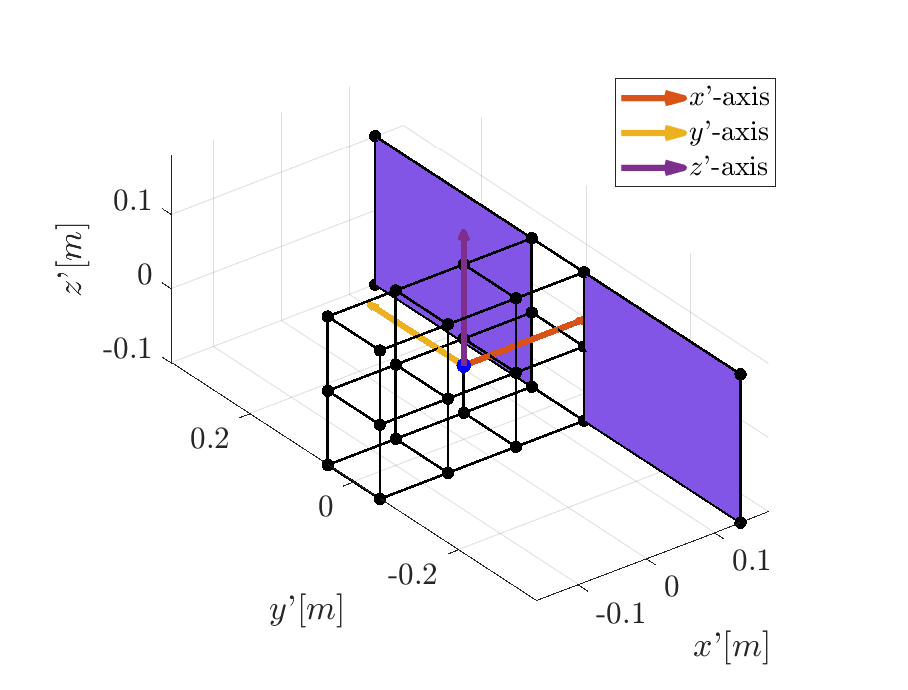
\includegraphics[width=0.7\textwidth]{graphics/cubesat.eps}
    \caption{Graphical representation of the 6U CubeSat}
    \label{fig:cubesat}
\end{figure}

\begin{table}[h]
    \centering
    \caption{Mass and dimensions of the satellite parts}
    \begin{tabular}{lcc}
    \toprule
    \toprule
    \textbf{Components} & \textbf{Mass} & \textbf{Dimensions} \\
    \midrule
    Main body & 6x 1 $kg$ & 0.3 x 0.2 x 0.1 $m$ \\
    \midrule
    Two solar panels & 2x 0.25 $kg$ & (2x) 0.3 x 0.2 x 0.005 $m$ \\
    \bottomrule
    \bottomrule
    \end{tabular}
    \label{tab:mass_dimensions}
\end{table}

\cref{fig:cubesat} also reports the frame of reference \{$x'$, $y'$, $z'$\}, placed in the geometrical centre of the satellite. In this frame of reference, the centre of gravity of the satellite has coordinates: $$ \mathbf{r}'_{CG} = \begin{bmatrix} 0.013 & 0 & 0 \end{bmatrix}^T\, m $$ These axes are parallel to the principal axes of inertia, which will be referred to as \{$x$, $y$, $z$\} (or body frame).

Considering the mass properties of the spacecraft and the dimensions of the components, the inertia matrix (referred to the CG in the principal axes) is equal to:

$$ I = \begin{bmatrix} 0.0504 & 0 & 0 \\
0 & 0.0771 & 0 \\
0 & 0 & 0.0841 
\end{bmatrix} kg \cdot m^2 $$

\subsection{Sensors}

The spacecraft is equipped with a Sun sensor, a star tracker and a magnetometer. The first two are used to generate measurements of the directions of celestial bodies, while the last one is sensible to Earth's magnetic field.

\subsubsection{Sun sensor}

The selected Sun sensor is the two-axis \textit{SSOC-D60} sensor, produced by \textit{SolarMems}. Its specifications are reported in \cref{tab:sun_sensor}.

\begin{table}[h]
    \centering
    \caption{SSOC-D60 specifications \cite{sun_sensor}}
    \begin{tabular}{cccccc}
    \toprule
    \toprule
    \textbf{Dimensions} & \textbf{Mass} & \textbf{FoV} & \textbf{Max. update rate} & \textbf{Accuracy} \\
    \midrule
    30 x 60 x 12 $mm$ & 35 $g$ & 120$^{\circ}$ ($\pm$60$^{\circ}$) & 50 $Hz$ & < 0.3$^{\circ}$ \\
    \bottomrule
    \bottomrule
    \end{tabular}
    \label{tab:sun_sensor}
\end{table}

The field of view is assumed to be conical. The sensor is placed on the top side of the spacecraft, next to the solar panels, so its coordinates in the \{$x'$, $y'$, $z'$\} frame are $\mathbf{r}'_{SS} = [0.15,\, 0,\, 0]^T \, m$. The sensor frame is aligned with the principal axes, so the rotation matrix from the body frame to the sensor frame $A_{s/b}^{SS}$ is simply the identity matrix $\mathbb{I}_3$

\subsubsection{Star tracker}

The chosen star tracker is \textit{arcsec}'s \textit{Sagitta}, whose specifications are reported in \cref{tab:star_tracker}. It can track up to 32 stars simultaneously and up to magnitude 6.

\begin{table}[h]
    \centering
    \caption{Sagitta specifications \cite{star_tracker}}
    \begin{tabular}{cccccc}
    \toprule
    \toprule
    \textbf{Dimensions} & \textbf{Mass} & \textbf{FoV} & \textbf{Max. update rate} & \multicolumn{2}{c}{\textbf{Accuracy}} \\
    \midrule
    \multirow{2}{*}{44 x 50 x 95 $mm$} & \multirow{2}{*}{250 $g$} & \multirow{2}{*}{40$^{\circ}$ ($\pm$20$^{\circ}$)} & \multirow{2}{*}{5 $Hz$} & cross-bore s. & roll-bore s. \\
    \cmidrule{5-6}
    & & & & 2" & 10"  \\
    \bottomrule
    \bottomrule
    \end{tabular}
    \label{tab:star_tracker}
\end{table}

The field of view is assumed to be conical. The position of the sensor in the \{$x'$, $y'$, $z'$\} frame is $\mathbf{r}'_{ST} = [-0.1,\, 0.05,\, 0]^T \,m$. The bore sight direction (considered to be the $1^{st}$ axis in the sensor frame) is coincident with the $y$-axis of the body frame, while the $3^{rd}$ axis is directed as $z$. The rotation matrix from the body frame to the sensor frame is therefore:

$$ A_{s/b}^{ST} = \begin{bmatrix}
0 & 1 & 0 \\
-1 & 0 & 0 \\
0 & 0 & 1
\end{bmatrix} $$

\subsubsection{Magnetometer}

The specifications of the selected magnetometer, \textit{NSS Magnetometer} by \textit{New Space Systems}, are presented in \cref{tab:magnetometer}. The sensor provides tri-axial measurements of the magnetic field.

\begin{table}[h]
    \centering
    \caption {NSS Magnetometer specifications \cite{magnetometer}}
    \begin{tabular}{ccccc}
    \toprule
    \toprule
    \textbf{Dimensions} & \textbf{Mass} & \textbf{Max. update rate} & \textbf{Noise density @} 1 $Hz$ & \textbf{Orthogonality} \\
    \midrule
    99 x 43 x 17 $mm$ & 85 $g$ & 18 $Hz$ & 16 $nT$ $rms/Hz$ & $\leq 1^{\circ}$ \\
    \bottomrule
    \bottomrule
    \end{tabular}
    \label{tab:magnetometer}
\end{table}

\subsection{Actuators}

The spacecraft is equipped with a magnetorquer and a set of four reaction wheels.

\subsubsection{Magnetorquer}

The chosen magnetorquer is the \textit{NanoTorque GST-600}, developed by \textit{GomSpace}. It is composed of three coils which generate magnetic dipoles in three orthogonal directions (which are, in this case, coincident with the axes of the body frame). Its properties are reported in \cref{tab:magnetorquer}.

\begin{table}[h]
    \centering
    \caption{GST-600 specifications \cite{magnetorquer}}
    \begin{tabular}{cccc}
    \toprule
    \toprule
    \multirow{2}{*}{\textbf{Dimensions}} & \multirow{2}{*}{\textbf{Mass}} & \textbf{Max. dipole strength} & \textbf{Max. dipole strength} \\
    & & ($x-$, $y-$axis) & ($z-$axis) \\
    \midrule
    90.5 x 96.9 x 17.2 $mm$ & 156 $g$ & 0.31 $A/m^2$ & 0.34 $A/m^2$ \\
    \bottomrule
    \bottomrule
    \end{tabular}
    \label{tab:magnetorquer}
\end{table}

\subsubsection{Reaction wheels}

The selected set of reaction wheels is the \textit{SatBus 4RW0} by \textit{NanoAvionics}. It consists of four identical wheels arranged in a pyramid configuration. The specifications of this product are reported in \cref{tab:reaction_wheels}.

\begin{table}[h]
    \centering
    \caption{SatBus 4RW0 specifications}
    \begin{tabular}{ccccc}
    \toprule
    \toprule
    \multirow{2}{*}{\textbf{Dimensions}} & \multirow{2}{*}{\textbf{Mass}} & \textbf{Inertia moment around} & \textbf{Max. torque} & \textbf{Max. momentum} \\
    & & \textbf{spin axis} (single wheel) & (single wheel) &  (single wheel) \\
    \midrule
    92.5 x 92.5 x 51.3 $mm$ & 665 $g$ & 3.24 $\cdot 10^{-5}\,kg\cdot m^2$ & 3.2 $mN \cdot m$ & $20 \, mN \cdot ms$ \\
    \bottomrule
    \bottomrule
    \end{tabular}
    \label{tab:reaction_wheels}
\end{table}